\documentclass[a4paper, 12pt]{article}
\usepackage[a4paper, margin=1in]{geometry}      % customize layout
\usepackage{mathptmx}                           % times roman font
\usepackage[T1]{fontenc}                        % enhance fonts
\usepackage[utf8]{inputenc}                     % special characters are usable now
\usepackage{microtype}                          % provides smooth text appearance and auto hyphenation
\usepackage{indentfirst}                        % indent after new section
\usepackage[english]{babel}                     % document language is english
\usepackage{mathtools}                          % rearranges the equations display geometry
\usepackage{paralist}                           % compact lists, customizable labels and layout options
\usepackage{graphicx}                           % include graphicals
\usepackage{xcolor}                             % now we have colors
\usepackage[section]{placeins}                  % causes an implicit \FloatBarries to be used at the beginning of each section, so figure dont float into another section
\usepackage{wrapfig}                            % lets text flow around a figure or a table: environments: wrapfigure, wraptable
\usepackage{subfig}                             % create subfigures
\usepackage[font=scriptsize]{caption}           % adjust caption font size
\usepackage{listings}                           % insert codeblocks
\usepackage{bookmark}                           % bookmarking
\usepackage{hyperref}                           % bookmarking
\usepackage{varioref}                           % introduces the functions \vref and \vpageref, smart \ref and \pageref
\usepackage{cleveref}                           % introduces the functions \cref, \crefrange, \cpageref, \cpagerefrange
\hypersetup{pdfauthor={Ali Uçar},
  pdftitle={Experiment 6 Report},
  pdfsubject={Collisions, Impulse and Momentum: Force and the Conservation of Linear Momentum},
  pdfkeywords={collision,impulse,momentum,physics}}

\definecolor{codegreen}{rgb}{0,0.6,0}
\definecolor{codegray}{rgb}{0.5,0.5,0.5}
\definecolor{codepurple}{rgb}{0.58,0,0.82}
\definecolor{backcolour}{rgb}{0.95,0.95,0.92}
\lstdefinestyle{mystyle}{
    backgroundcolor=\color{backcolour},   
    commentstyle=\color{codegreen},
    keywordstyle=\color{magenta},
    numberstyle=\tiny\color{codegray},
    stringstyle=\color{codepurple},
    basicstyle=\ttfamily\footnotesize,
    breakatwhitespace=false,         
    breaklines=true,                 
    captionpos=b,                    
    keepspaces=true,                 
    numbers=left,                    
    numbersep=5pt,                  
    showspaces=false,                
    showstringspaces=false,
    showtabs=false,                  
    tabsize=2
}
\lstset{style=mystyle}

% \usepackage{parskip}                          % do not auto-indent paragraphs
% \usepackage[singlespacing]{setspace}          % line spacing
% \usepackage{index} \makeindex                 % indexing
% \usepackage{array}                            % introduces customizable layout variables
% \setlength{\extrarowheight}{4pt}              % row height for tables, comes with array package
% \usepackage{booktabs}                         % provides \toprule[thickness] etc. for tables

% section = section* --- for bookmarking purposes
\makeatletter
\renewcommand\@seccntformat[1]{}
\makeatother
\newcommand{\head}[1]{\section{\normalsize \textit #1}}
\newcommand{\subhead}[1]{\subsection{\normalsize #1}}

\begin{document}

    \title{Title}
    \author{Author}
    \date{\today}
    % \maketitle

    \noindent
    \textbf{Name Surname:} Ali Uçar
    \hfill \textbf{Date:} \today \\
    \textbf{Student ID No:} 2555555
    \hfill \textbf{Signature:} \\
    \textbf{Section No:} 1 - Lab Sec. 6

    \begin{center}
        \head{Exp. 6: Collisions, Impulse and Momentum: Force and the Conservation of Linear Momentum}
    \end{center}

    \subhead{Abstract}
    In this experiment, conservation of momentum and conservation of energy were analyzed for two
    different scenarios under ideal circumstances. These ideal scenarios are which a collision happens for
    such inelastic and elastic collision. For elastic and inelastic collisions, pre-collision momentum and the
    post-collision momentum will be compared computationally. Similarly, same comparison has been
    established for the total kinetic energy before collision and the total kinetic energy after collision.

    \subhead{Introduction}
    An air track was used to provide a frictionless surface for which the blocks of mass could slide on, 
    where the two blocks of mass were placed on a straight line of air track. For part A of the experiment, 
    two blocks will be provided with a constant speed to make an elastic collision, which they do not crash 
    but conserve the mechanical energy within the system. By using motion sensors, functions of motions 
    of each car was produced. For part B of the experiment, inelastic collision of two blocks of mass was 
    examined, which they crash and stick with each other. Functions of motions with respect time was 
    produced with the same methodology.

    \subhead{Theory}
    The linear momentum of a particle is defined as the product of its mass and velocity.
    \begin{equation}
        \vec{p} = m \vec{v}
    \end{equation}
    The change in the momentum means that there is a change in the mass or velocity of the particle. In the
    experiment or general computation, there is no change in mass, so the equation extends as follows,
    where we can derive the force $\vec{F}$.
    \begin{equation}
        \vec{F} = \frac{d\vec{p}}{dt}
    \end{equation}
    Which means that the force applied over a period of time is equal to the change in the momentum, which
    is named as impulse.
    \begin{equation}
        \int F dt = \int dp = \Delta p = J
    \end{equation}
    In a system of particles, total momentum of the system is conserved (Burko, 2019).
    \begin{equation}
        \vec{p}_{\textnormal{total}} = \sum \vec{p}_i
        \label{eq:conserve_p}
    \end{equation}
    If the collision is elastic, the total kinetic energy of the system is conserved (Burko, 2019).
    \begin{equation}
        K_{total} = \sum K_i
        \label{eq:conserve_K}
    \end{equation}
    Kinetic energy is only conserved in elastic collisions, provided that the system has no external force
    applied on, collisions can be computed by using the concept of conservation of momentum. Inelastic
    collisions on the other hand, does not obey the conservation of kinetic energy rule because the system
    looses its mechanical energy, so for the inelastic collisions, $K_{\textnormal{initial}} > K_{\textnormal{final}}$.

    \subhead{Method and Description of Experiment}
    The experiment was set for measuring and comparing the pre-collision momentum and post-collision 
    momentum with respect to conservation of energy model. An air track was used as a flat surface for 
    which the both cars with masses $m_1 = 210~g$ and $m_2 = 220~g$ were provided with a constant speed by 
    applying a small force by hand where they had a velocity vector with opposite directions, so a collision 
    was happened with two objects not attaching to one another but repelling instantaneously. For another 
    perspective to part A, one block of mass was happened to be at rest with no velocity relative to the 
    ground reference frame, and the other block of mass hit the one that is at rest. These elastic collisions 
    was recorded by the motion sensors for the production of functions of motion with respect to time. So 
    the elastic collision is examined with respect to displacements and time passed. Obtained data was used
    to plot the graphs of position versus time $x_{(t)}$ for each object of mass of before and after the collision.
    For part B of the experiment, the same two blocks of masses were used with the same methodology 
    except the objects are modified with a pin and cushion accessory, this modification provided the system
    to perform an inelastic collision and blocks of masses was tied to together after the collision, meaning 
    that the final velocity for inelastic collision was happened to be the same for each block of mass.
    Finally, for part A and part B, pre-collision, post-collision and conservation of momentum was 
    compared.

    \subhead{Results}
    \begin{wrapfigure}{l}{0.25\textwidth}
        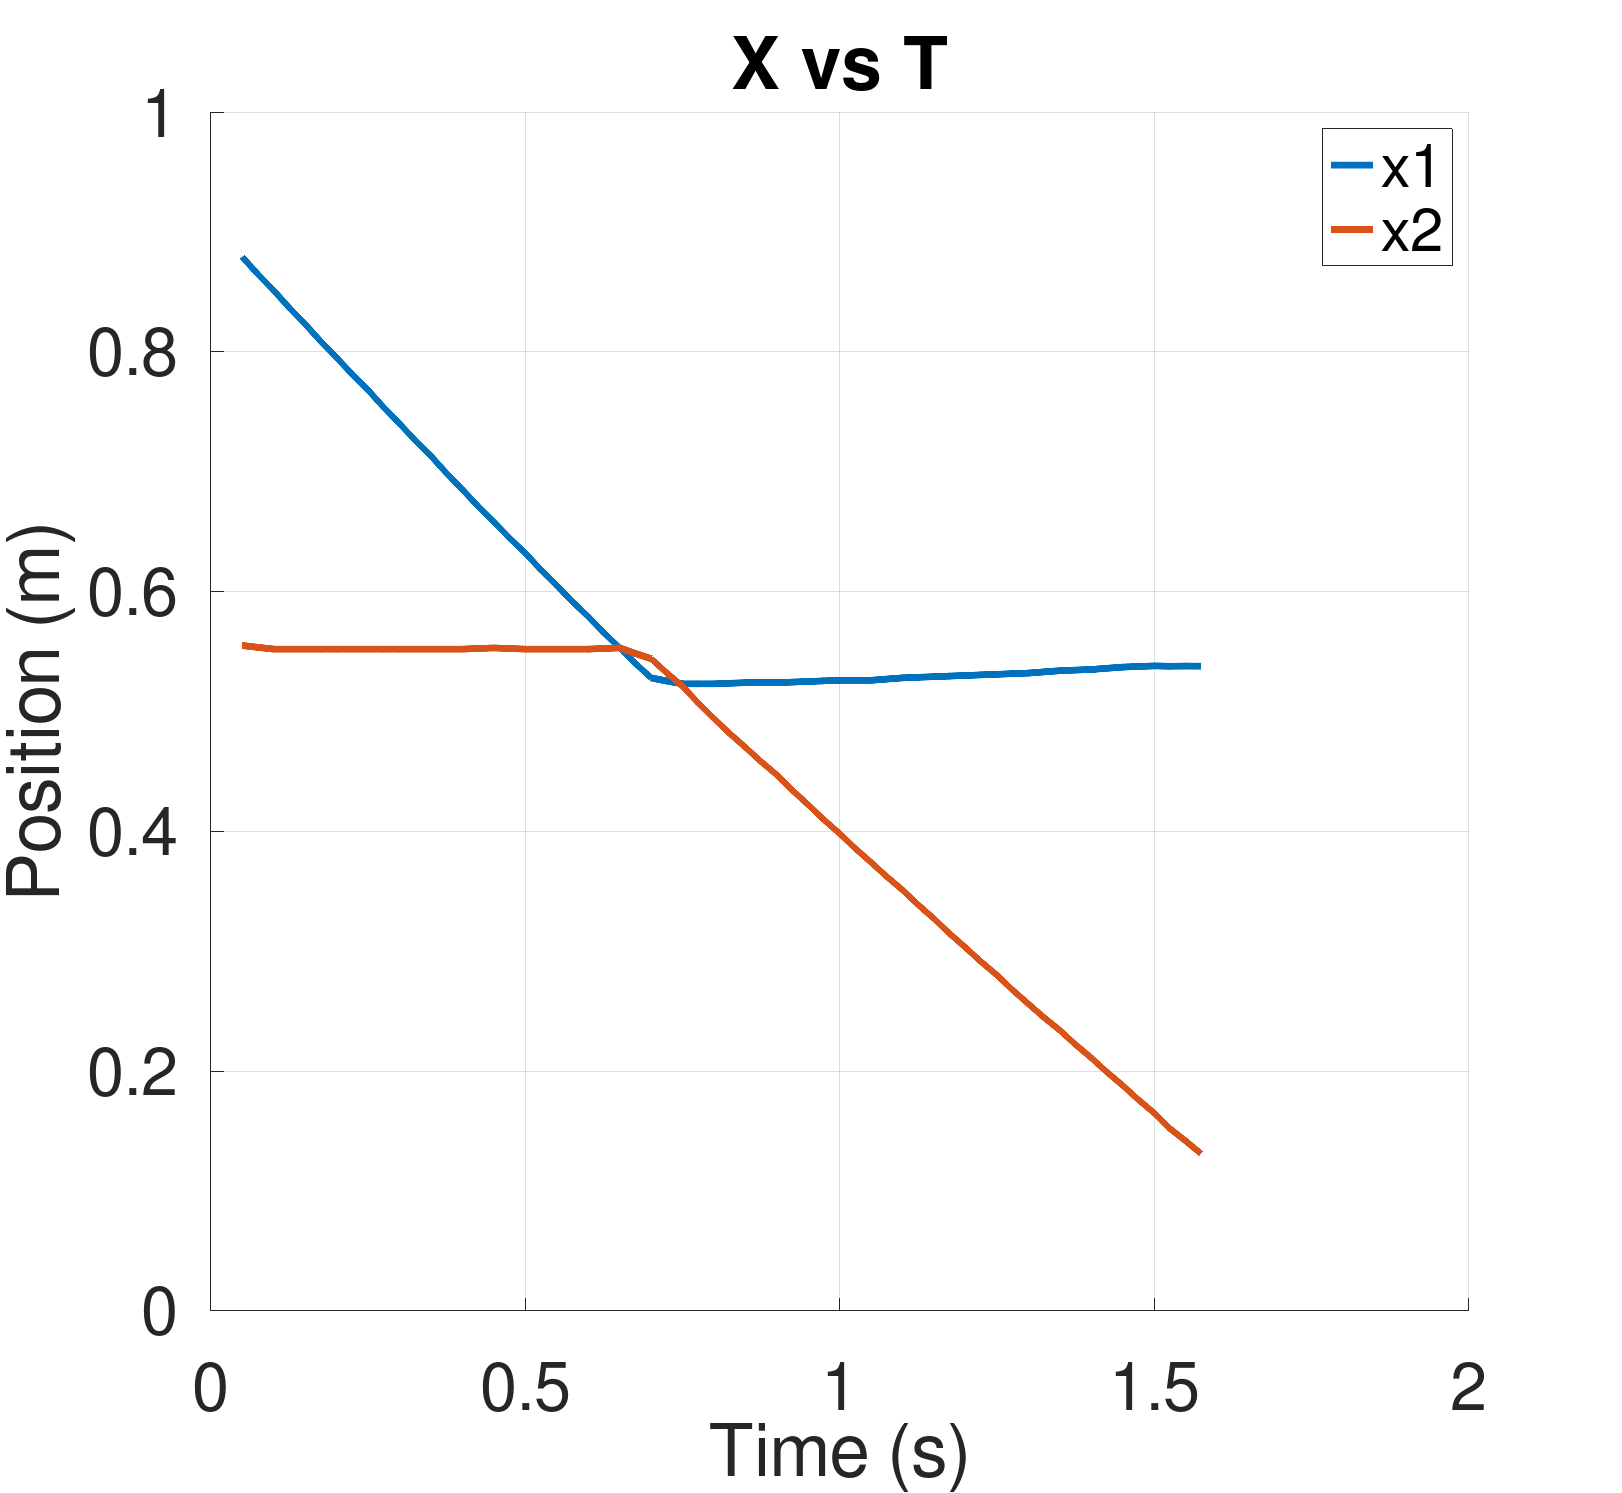
\includegraphics[width=0.25\textwidth]{./elastic_static_X.png}
        \caption{Position vs. time graph of part A, elastic static collision}
        \label{fig:elastic_static_X}

        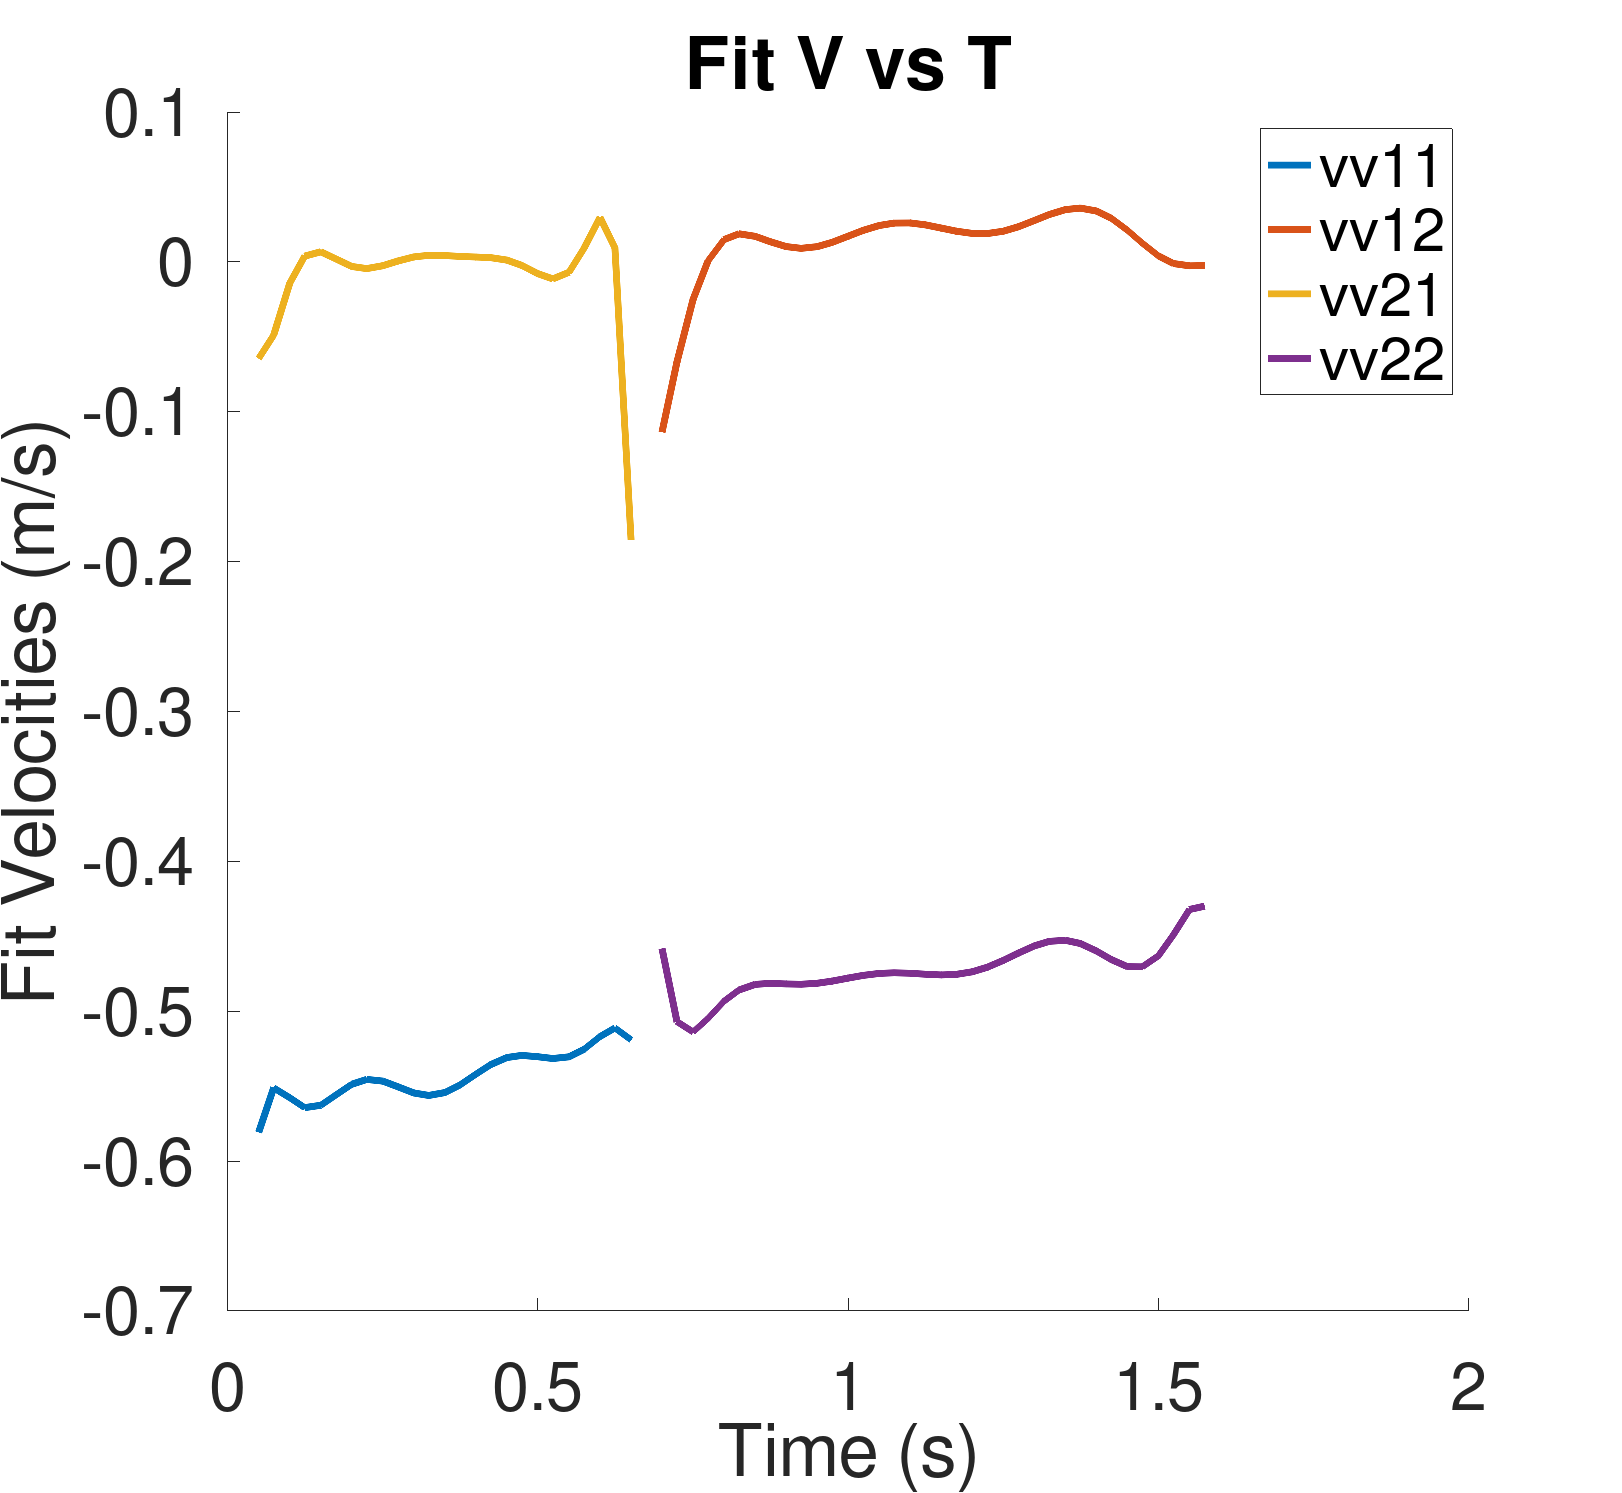
\includegraphics[width=0.25\textwidth]{./elastic_static_Vfit.png}
        \caption{Best fit velocity vs. time graph of part A, elastic static collision}
        \label{fig:elastic_static_V}
    \end{wrapfigure}
    For part A of the experiment, the graph of position versus time $x_{(t)}$ for two blocks of masses
    $m_1 = 210~g$ and $m_2 = 220~g$ represented. We divided the elastic collision part into two subsections
    for which the scenarios are firstly, one block of mass stays at rest and the other one proceeds its 
    motion with a constant velocity which performs a static collision; secondly, both blocks of
    masses have velocities with opposite directions to provide a dynamic collision. \\
    For the static collision section of part A, position versus time graph for both blocks of masses
    is shown in \cref{fig:elastic_static_X}, velocity vs. time graph is shown in \cref{fig:elastic_static_V}
    with best fit for pre-collision and post-collision. As seen in \cref{fig:elastic_static_V}, $m_1$ has a
    speed of $v_1 = -0.52~m/s$ and $m_2$ is stationary, which means $v_2 = 0$. After the collision, $m_1$ goes
    stationary with a speed of $v_1 = 0$, and $m_2$ has nearly the same speed as $v_2=-0.50~m/s$. For the
    \cref{eq:conserve_p} and \cref{eq:conserve_K}, the values are satisfied.

    For the dynamic collision of part A, position versus time graph is shown in \cref{fig:elastic_dynamic_X}.
    Velocity vs. time graph is shown in \cref{fig:elastic_dynamic_V} with best fit for pre-collision and
    post-collision. Initial velocity was given at first second and the collision happened after 0.5 seconds.
    As seen in \cref{fig:elastic_dynamic_V} $m_1$ has a speed of $v_1 = -0.80~m/s$, and $m_2$ has a speed of
    $v_2 = 0.50~m/s$. After the collision, $m_1$ has a speed of $v_1 = 0.45~m/s$ and $m_2$ has a speed of
    $v_2 = -0.75~m/s$; which again, satisfies \cref{eq:conserve_p} and \cref{eq:conserve_K}.

    \begin{wrapfigure}{o}{0.25\textwidth}
        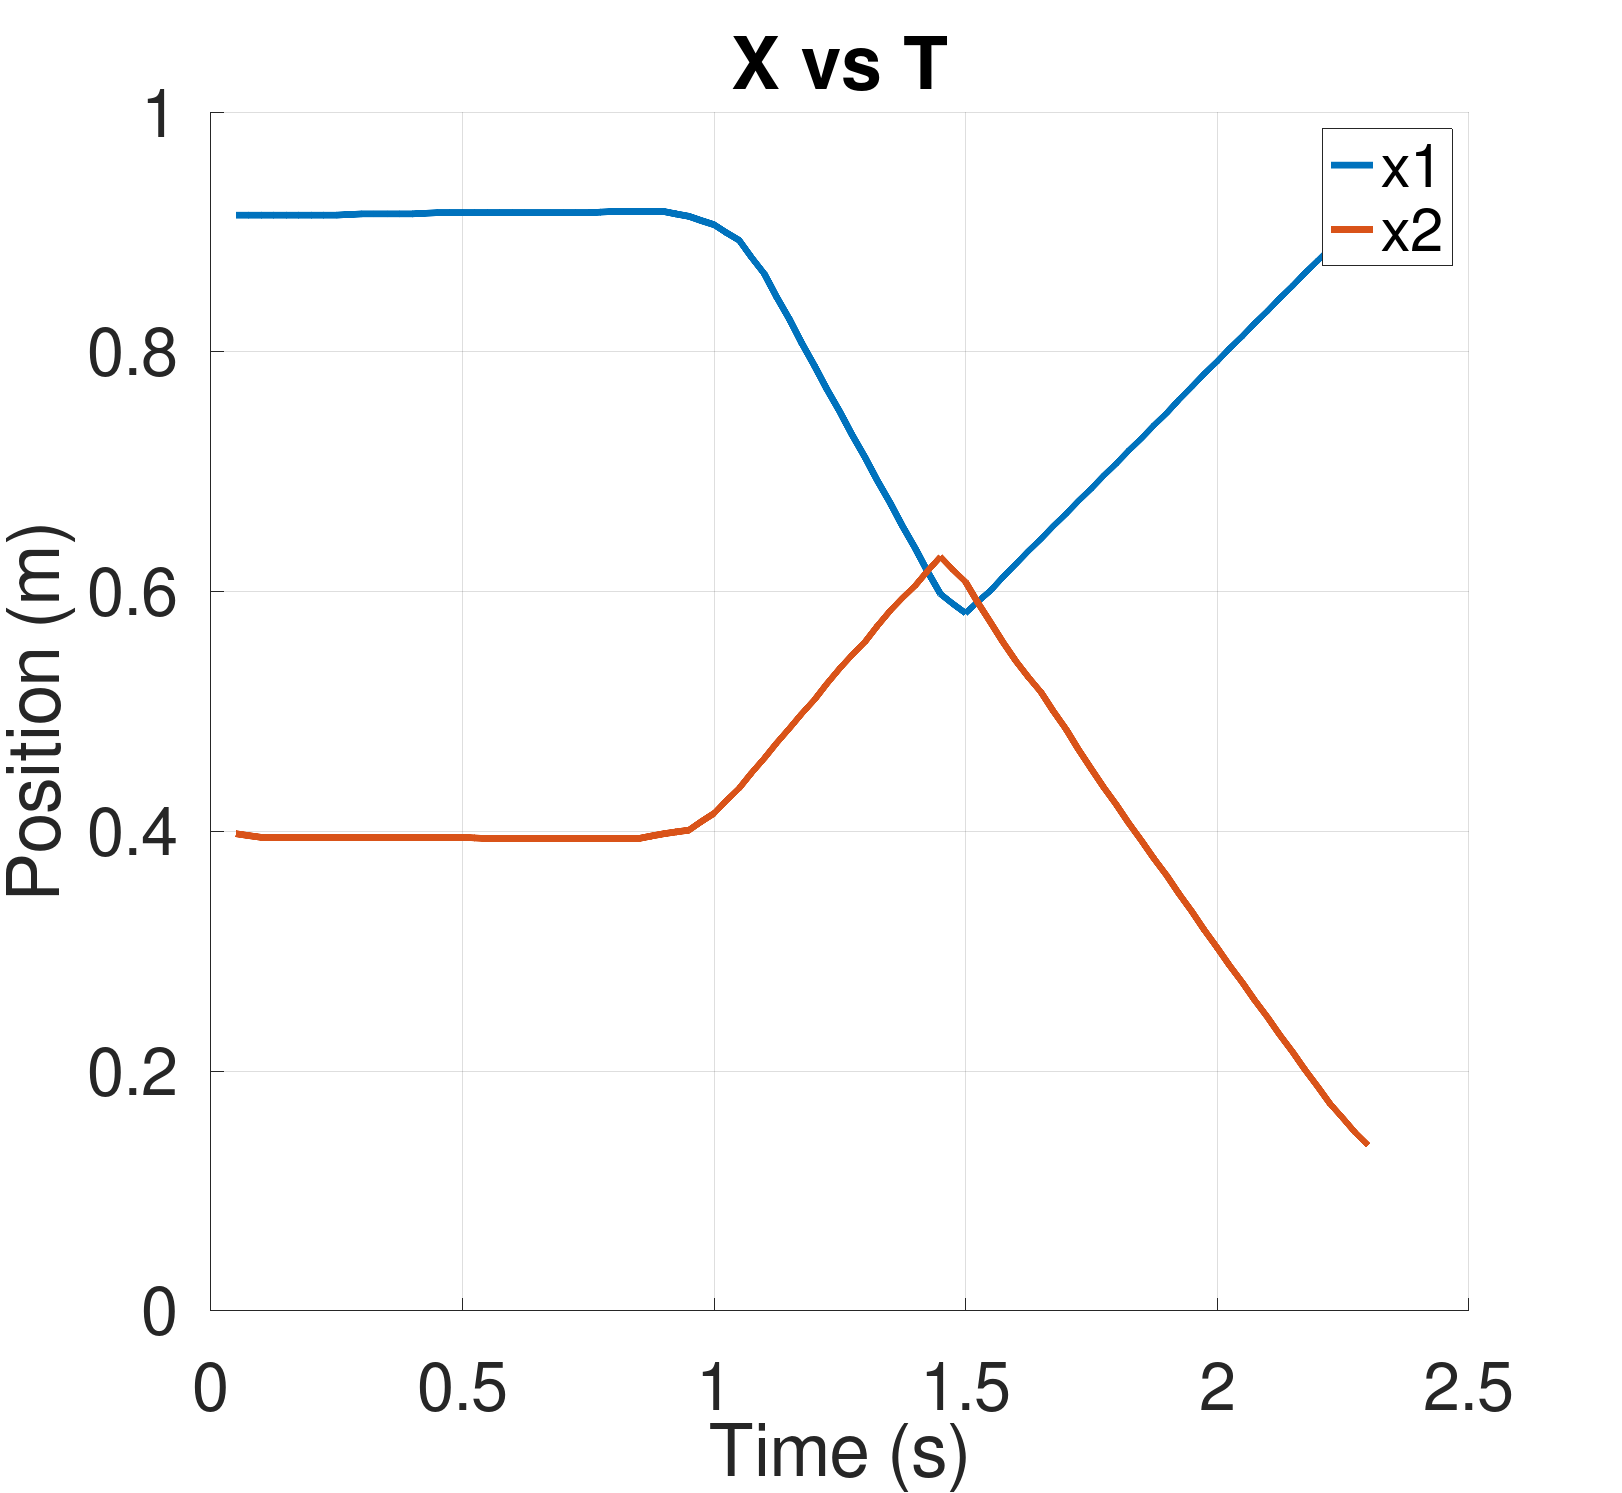
\includegraphics[width=0.25\textwidth]{./elastic_dynamic_X.png}
        \caption{Position vs. time graph of part A, elastic dynamic collision}
        \label{fig:elastic_dynamic_X}

        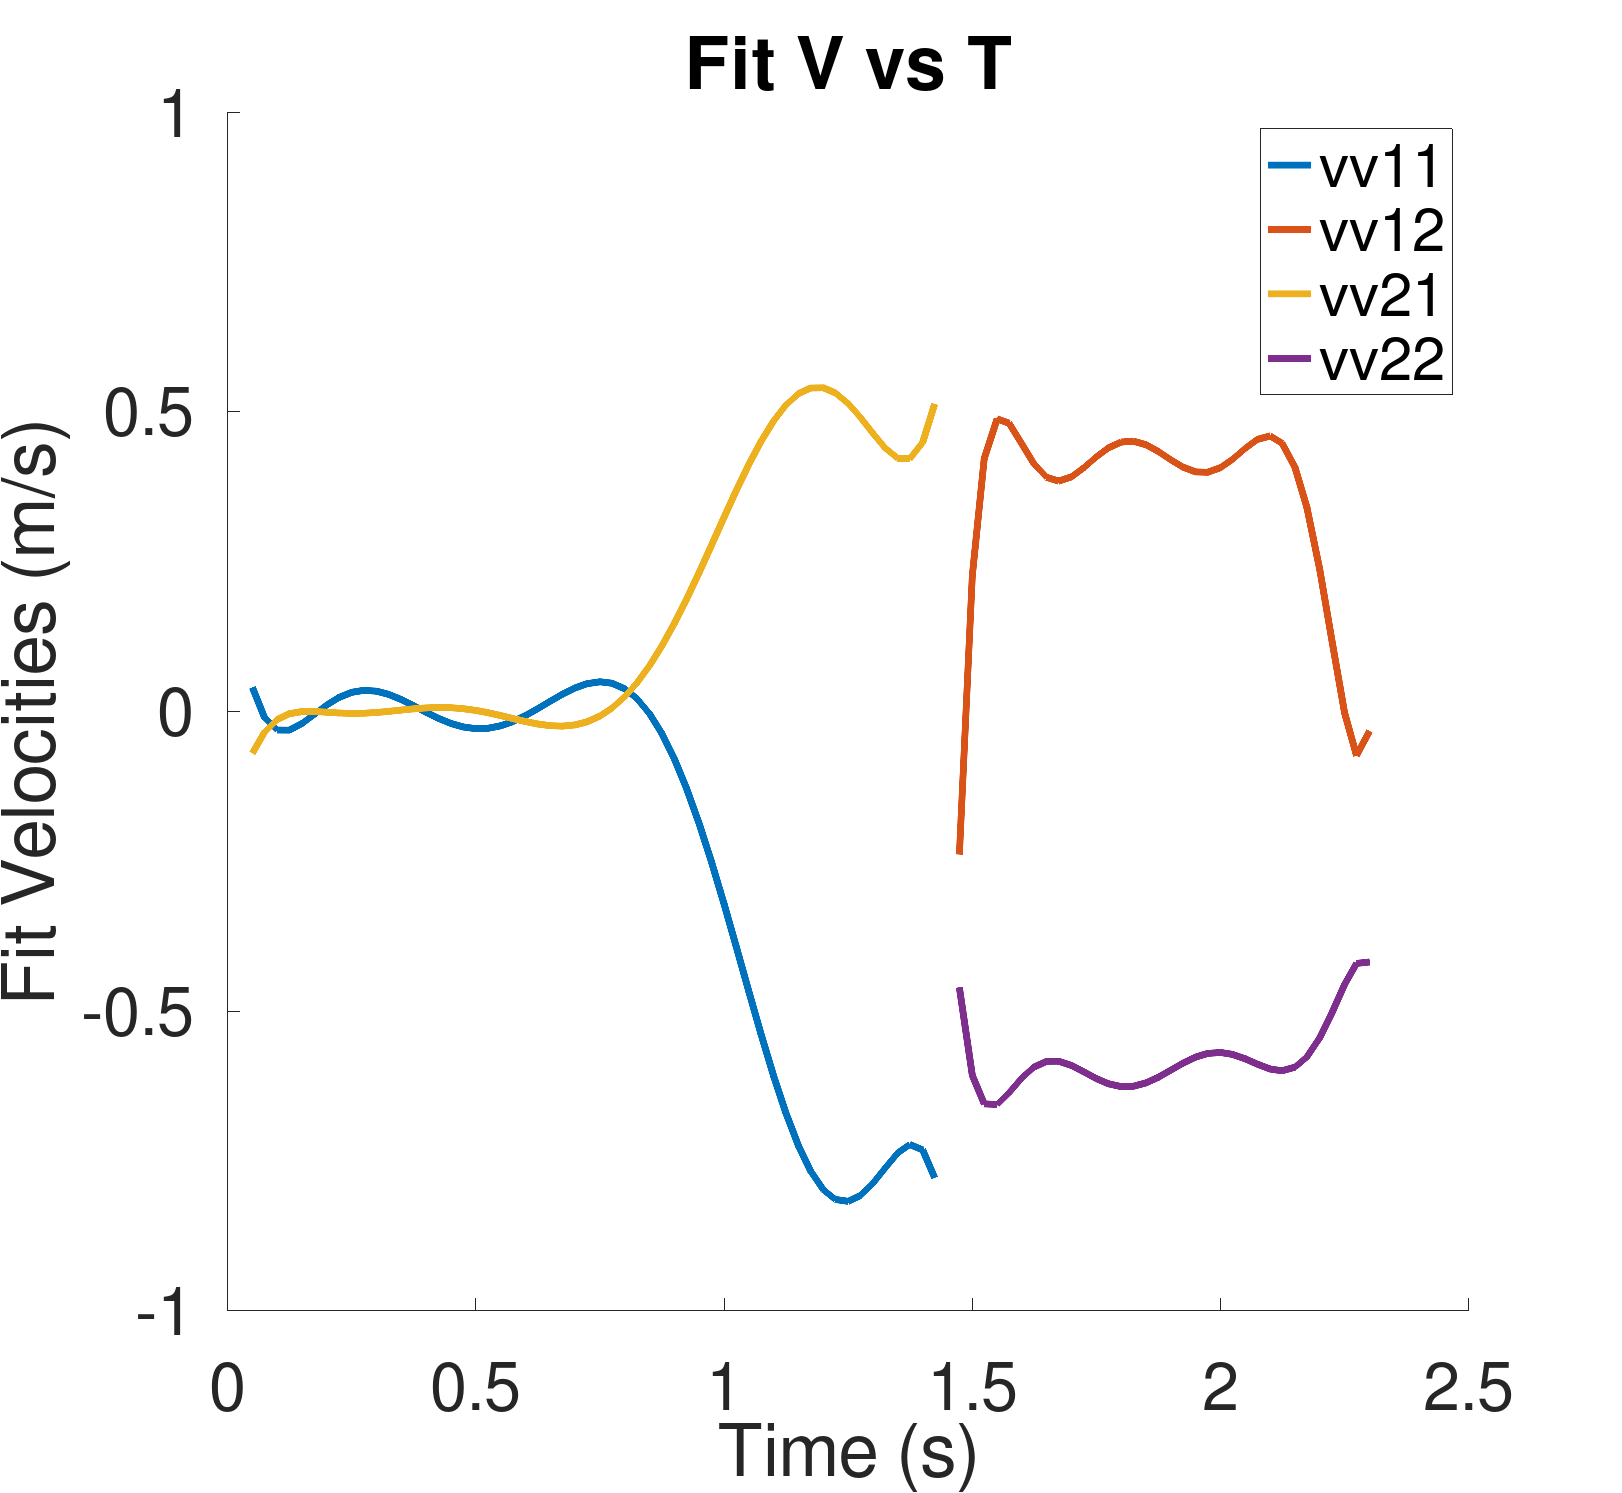
\includegraphics[width=0.25\textwidth]{./elastic_dynamic_Vfit.png}
        \caption{Best fit velocity vs. time graph of part A, elastic dynamic collision}
        \label{fig:elastic_dynamic_V}
    \end{wrapfigure}

    \newpage

    For part B of the experiment, inelastic collision is divided into two parts,
    first one is static, one block of mass stays at rest and the other one proceed 
    its motion with a constant velocity which performs a static collision; 
    secondly, both blocks of masses have velocities with opposite directions to provide a dynamic collision.

    For the static collision of part B, position versus time graph for both block of masses is shown in 
    \cref{fig:inelastic_static_X}. Velocity versus time graph is shown in \cref{fig:inelastic_static_V} with best 
    fit for pre-collision and post-collision. As seen in \cref{fig:inelastic_static_V}, $m_1$ is stationary
    with a speed of $m_1 = 0$ and $m_2$ has a speed $v_2 > 0.60~m/s$. After collision, the speed of 
    the mass $m_1 + m_2$ is around $v_f = 0.30~m/s$, which satisfies the \cref{eq:conserve_p} but not \cref{eq:conserve_K}.

    For the dynamic collision of part B, position versus time graph for both block of masses is 
    shown in \cref{fig:inelastic_dynamic_X}. Velocity versus time graph is shown in \cref{fig:inelastic_dynamic_V} 
    with best fit for pre-collision and post-collision. As seen on \cref{fig:inelastic_dynamic_V}, $m_1$
    has a speed of $v_1 = 0.78~m/s$ and $m_2$ has a speed of $v_2 = -0.60~m/s$. After the collision, 
    the speed of the mass $m_1 + m_2$ is around $v_f = 0$.

    \bigskip
    \bigskip
    \begin{figure}[ht]
        \begin{minipage}{0.40\textwidth}
            \centering
            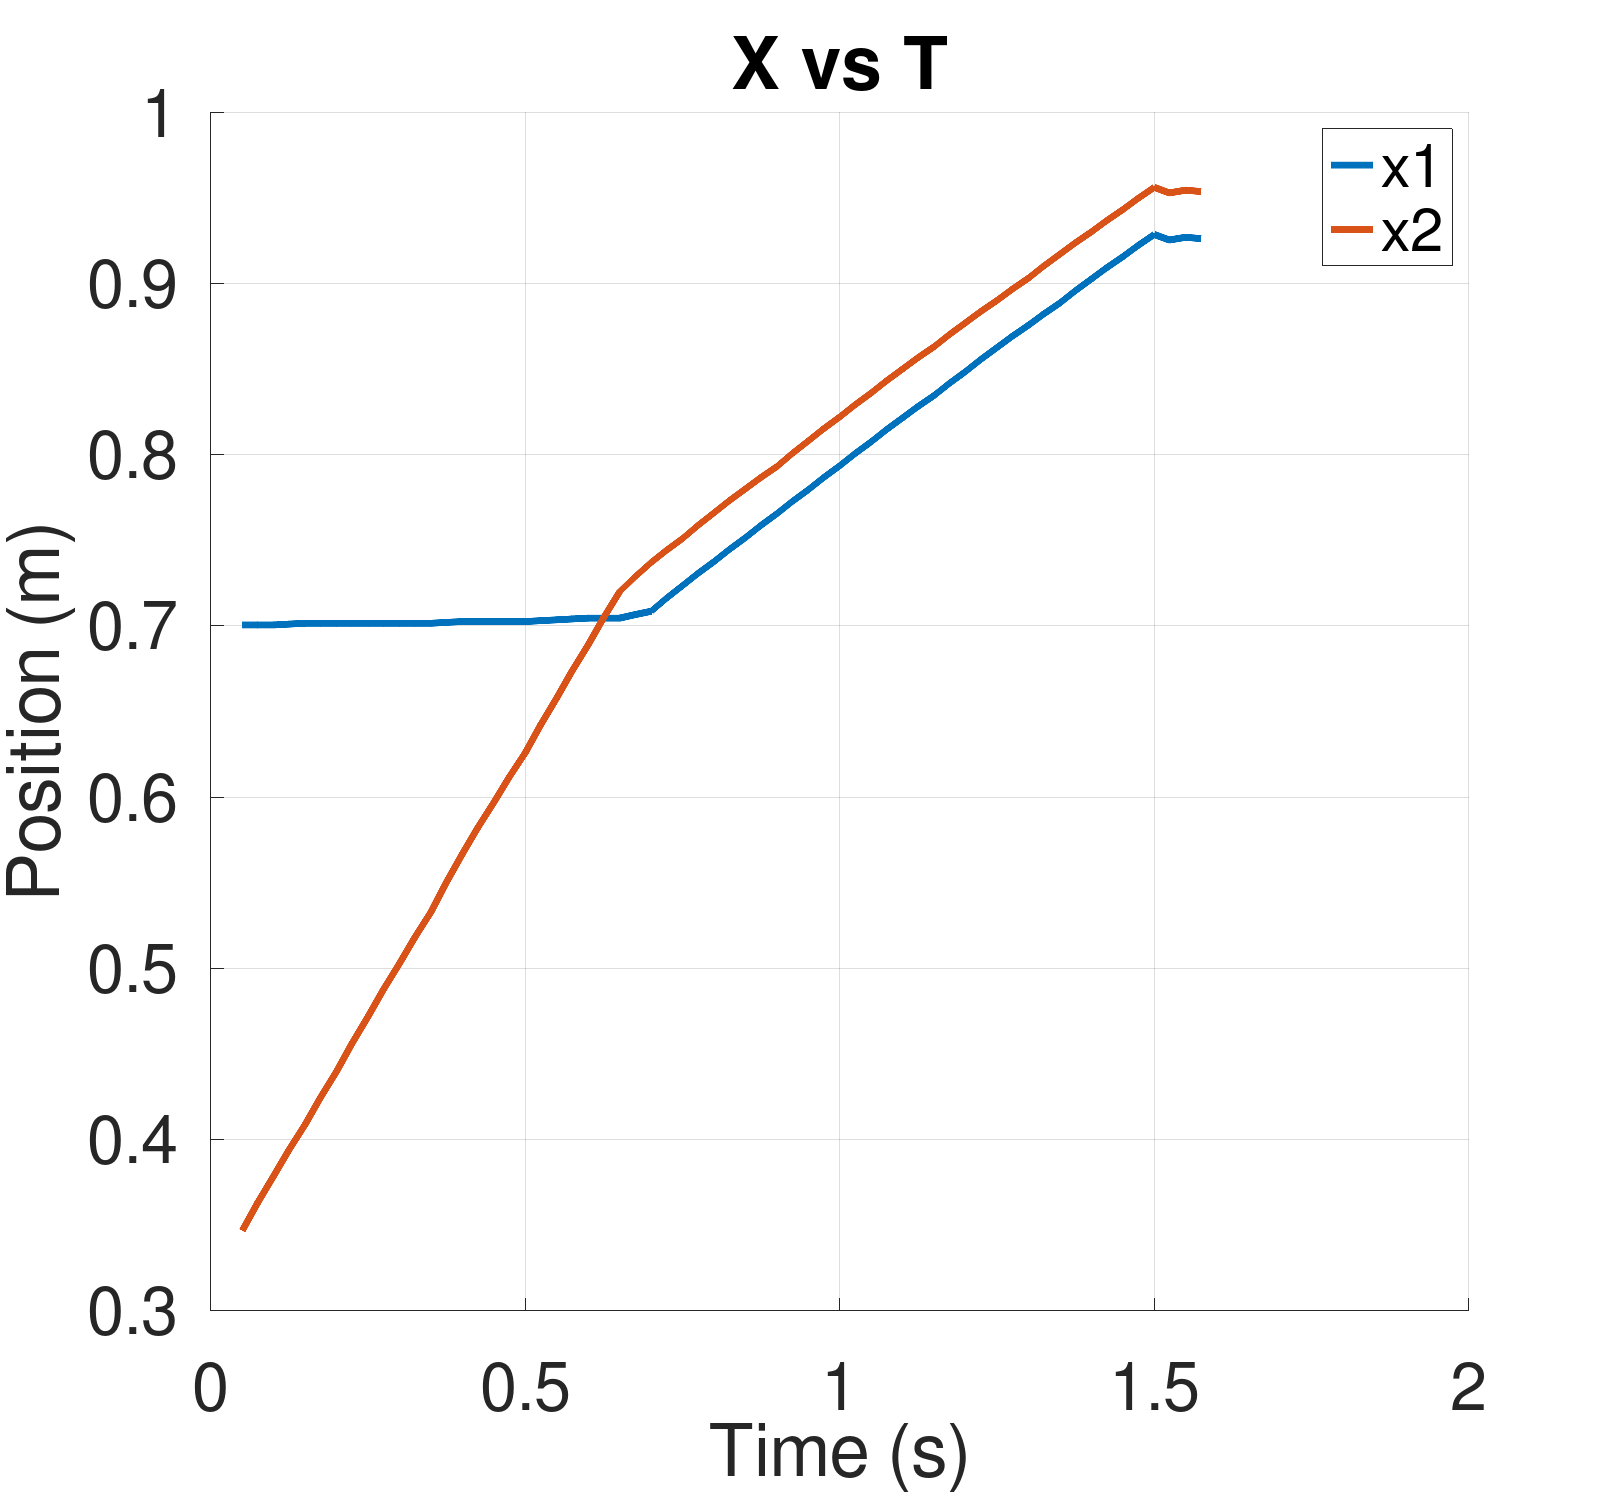
\includegraphics[width=\linewidth]{./inelastic_static_X.png}
            \caption{Position vs. time graph of part B, inelastic static collision}
            \label{fig:inelastic_static_X}
        \end{minipage}
        \hfill
        \begin{minipage}{0.40\textwidth}
            \centering
            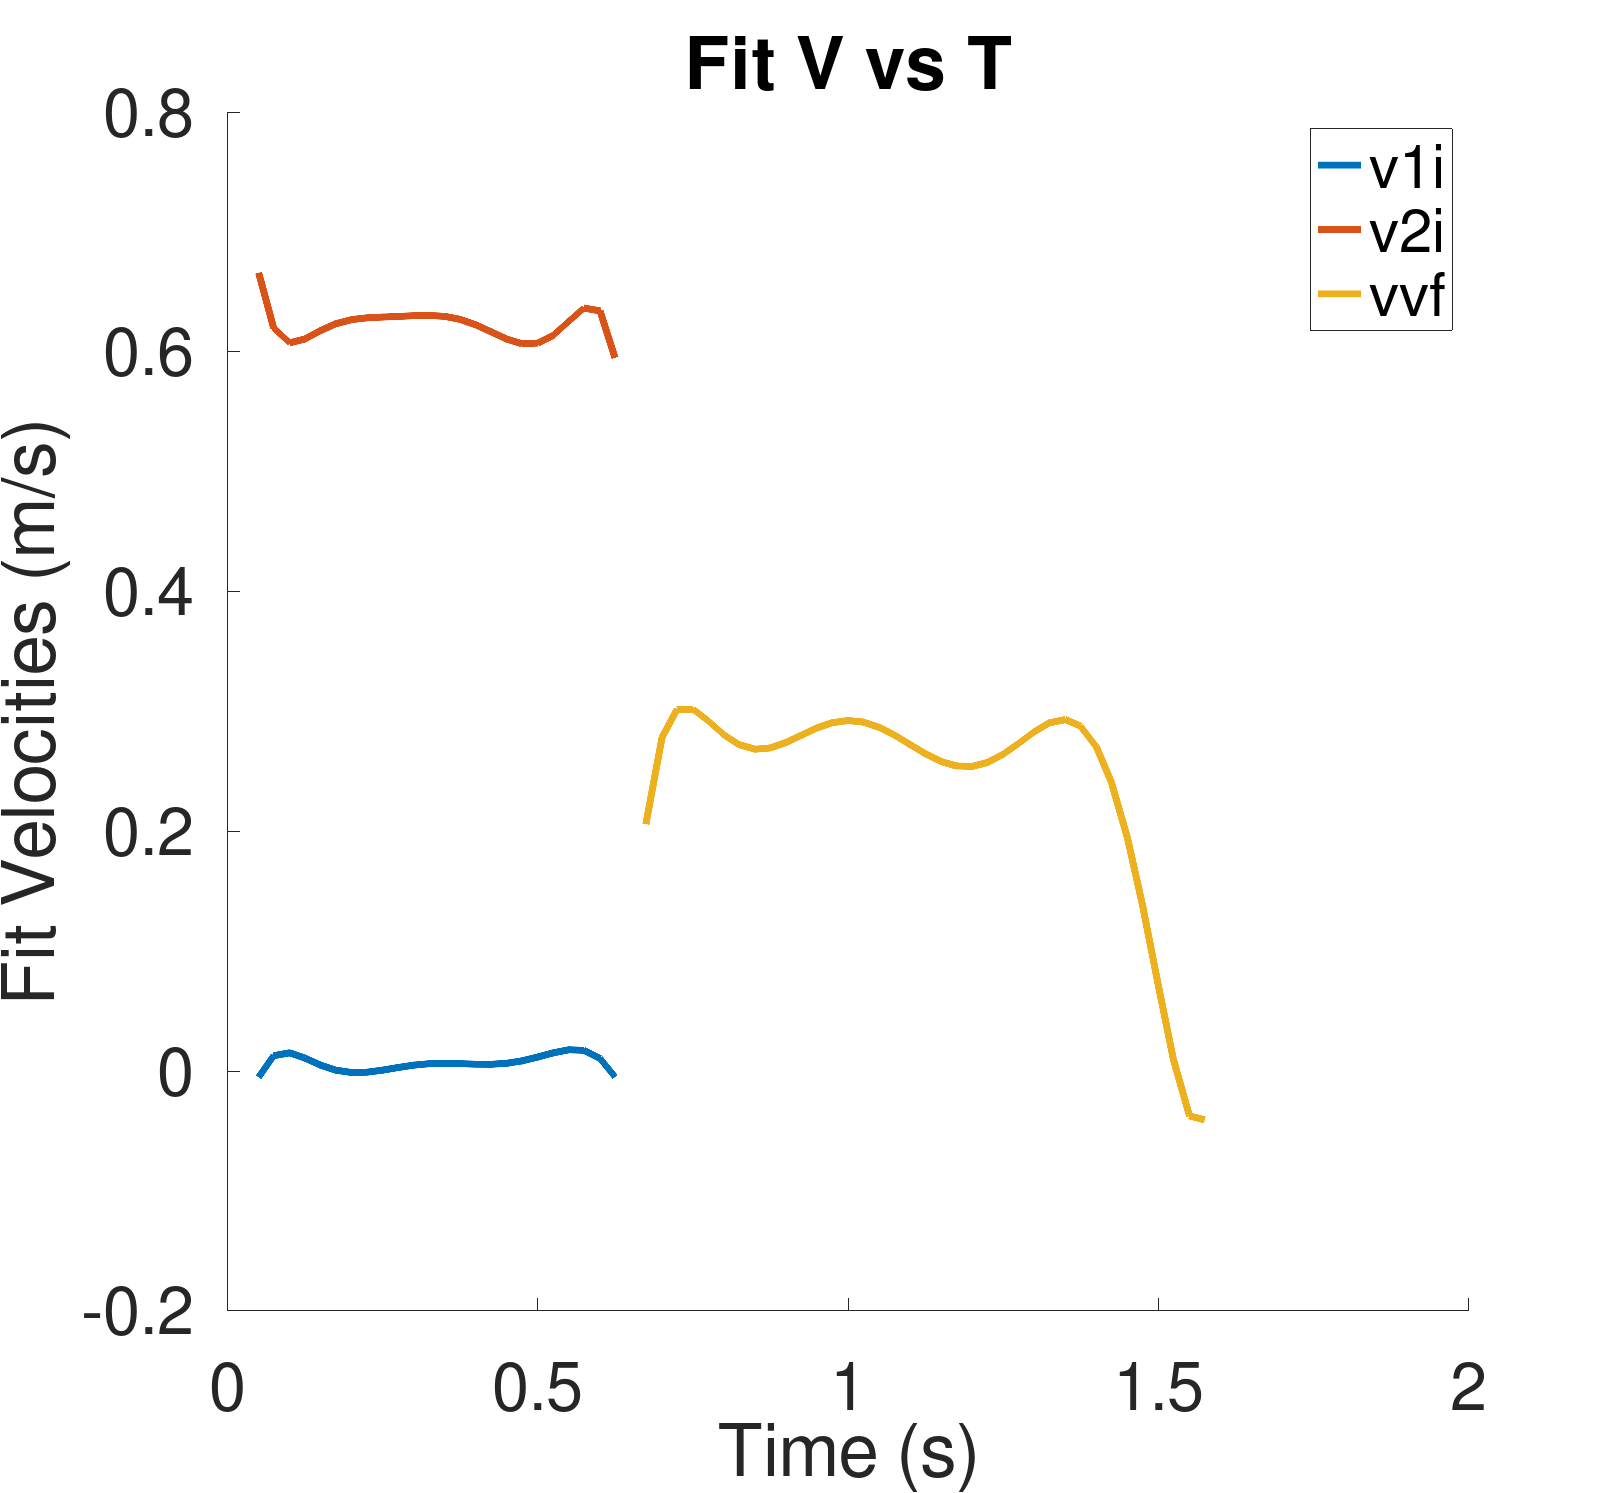
\includegraphics[width=\linewidth]{./inelastic_static_Vfit.png}
            \caption{Best fit velocity vs. time graph of part B, inelastic static collision}
            \label{fig:inelastic_static_V}
        \end{minipage}
    \end{figure}
    \begin{figure}[ht]
        \begin{minipage}{0.35\textwidth}
            \centering
            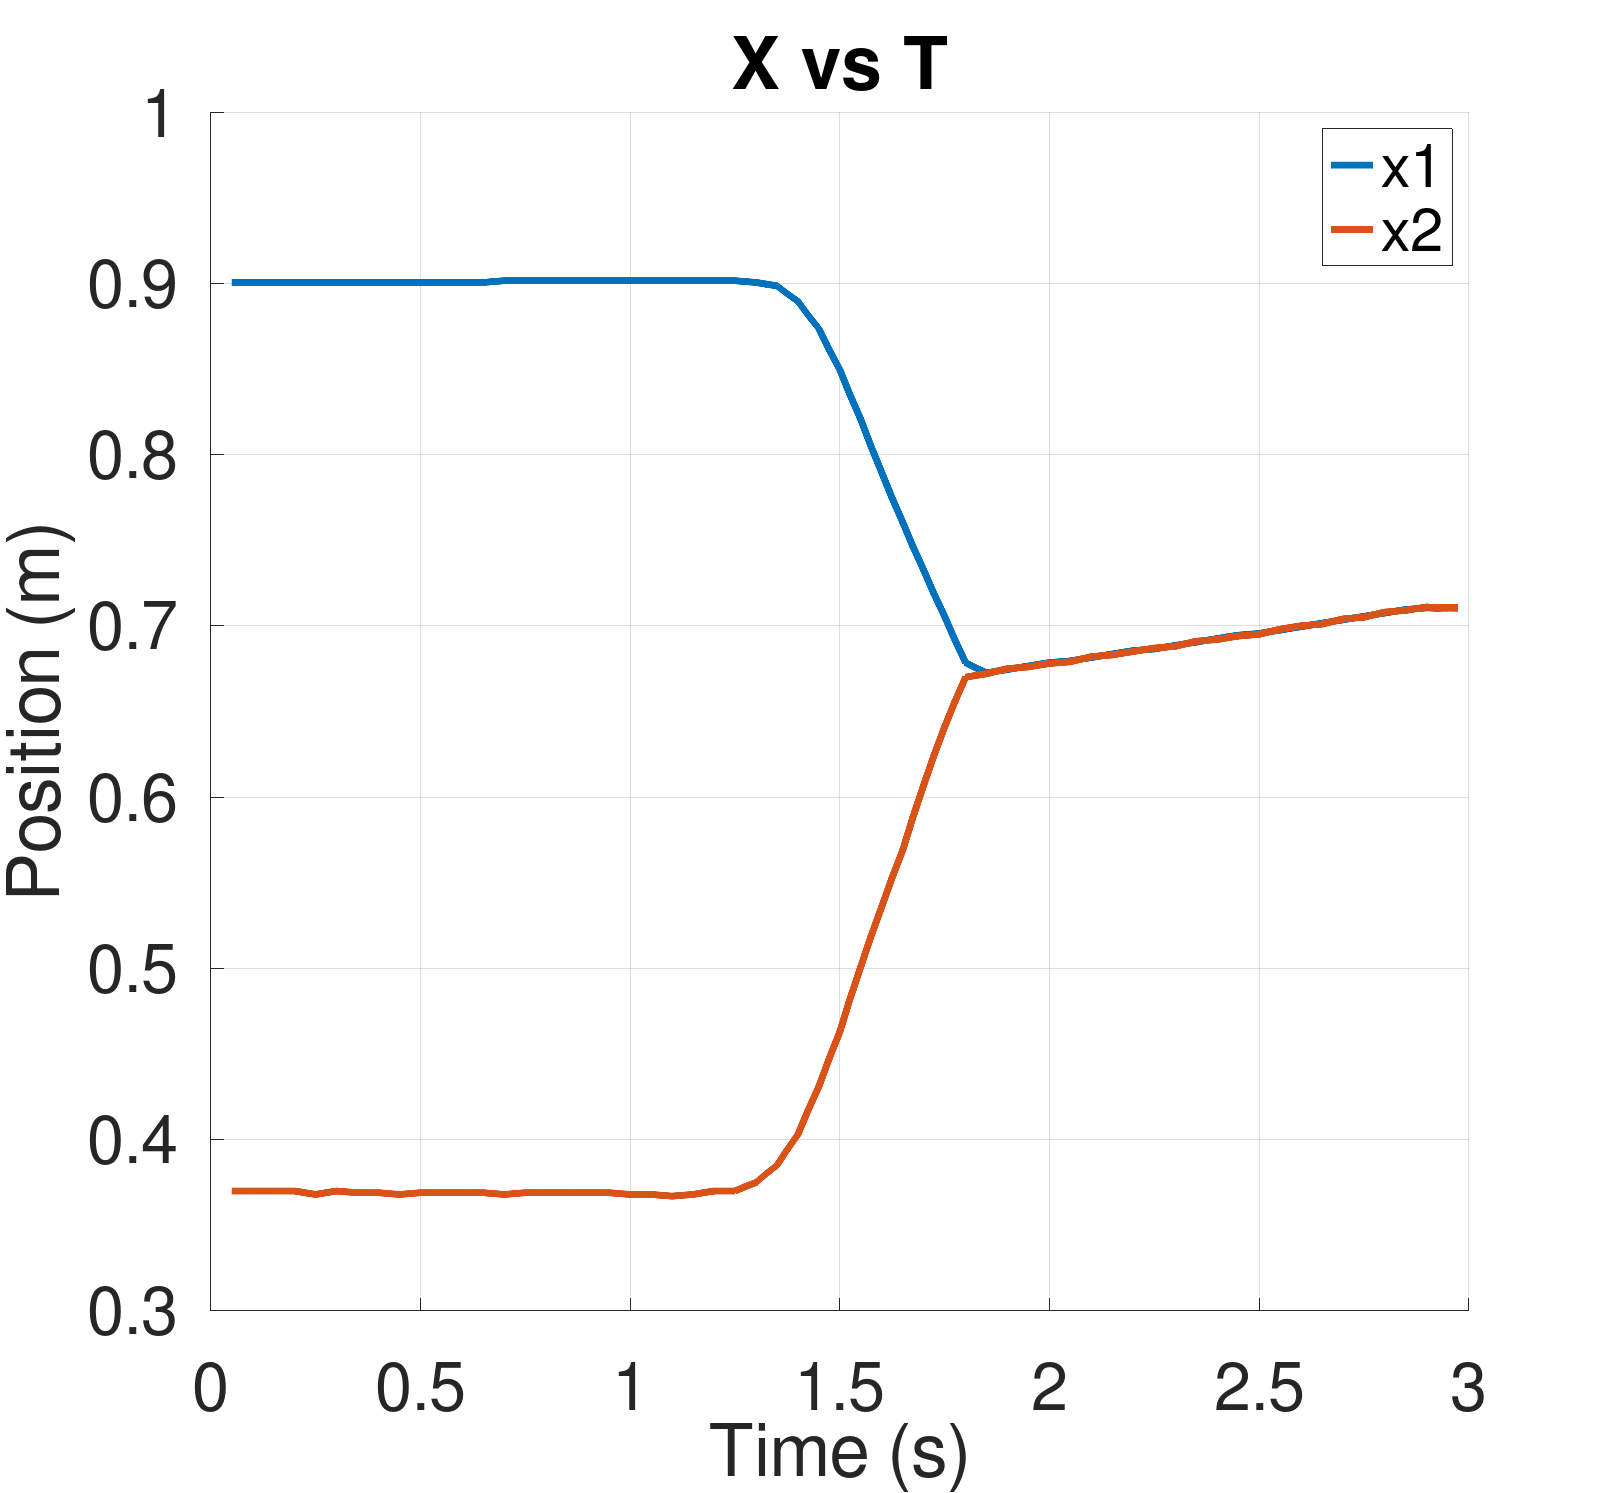
\includegraphics[width=\linewidth]{./inelastic_dynamic_X.png}
            \caption{Position vs. time graph of part B, inelastic dynamic collision}
            \label{fig:inelastic_dynamic_X}
        \end{minipage}
        \hfill
        \begin{minipage}{0.35\textwidth}
            \centering
            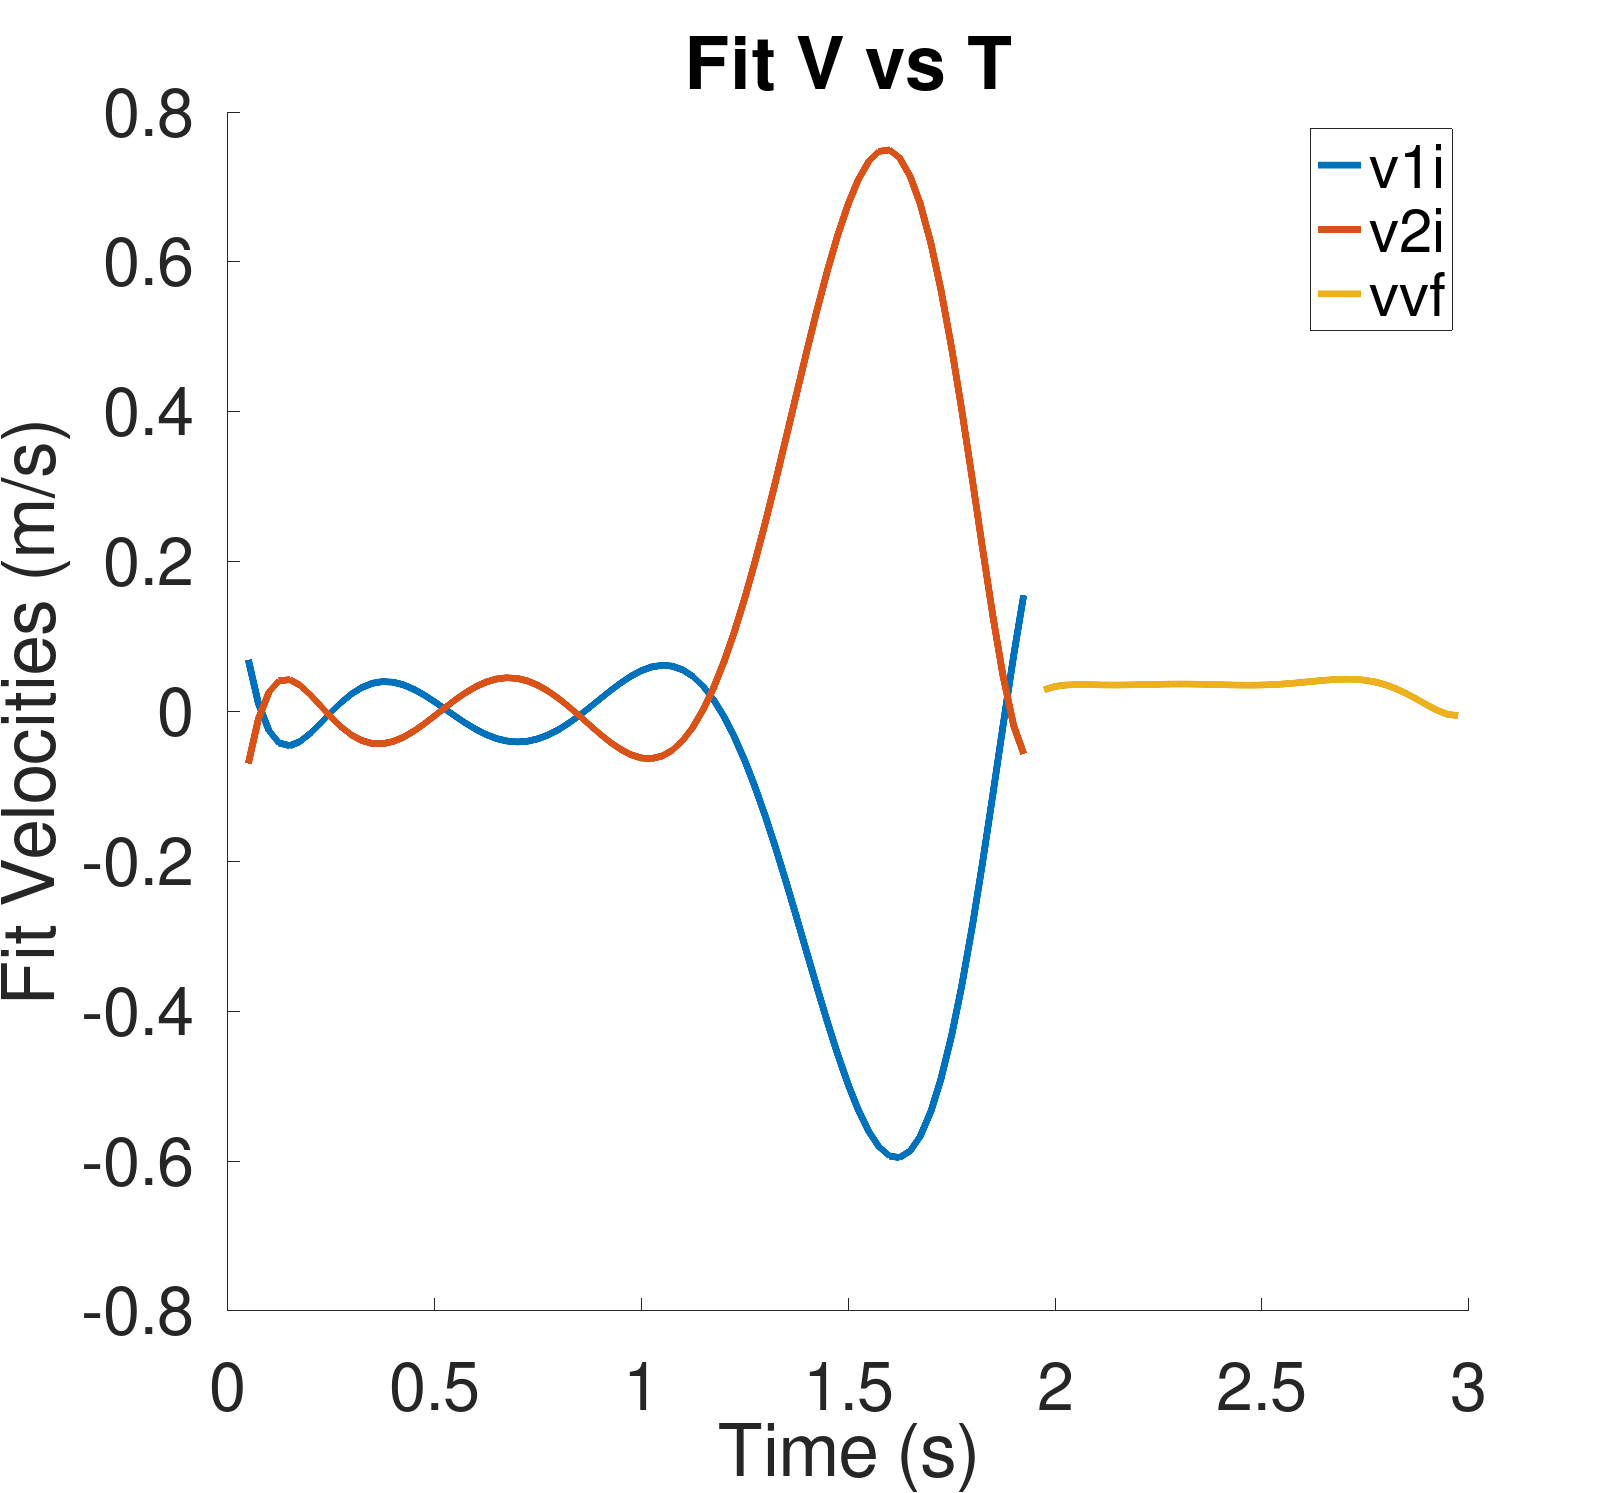
\includegraphics[width=\linewidth]{./inelastic_dynamic_Vfit.png}
            \caption{Best fit velocity vs. time graph of part B, inelastic dynamic collision}
            \label{fig:inelastic_dynamic_V}
        \end{minipage}
    \end{figure}
    \newpage
    \noindent
    The possible errors and their estimations are:
    \begin{itemize}
        \item Motion sensor’s uncertain accuracy rates (Cannot be quantified.)
        \item No ideal insurance for frictionless surface provided by air track (Cannot be quantified.)
        \item Error in computations (Cannot be quantified.)
    \end{itemize}
    \subhead{Conclusions}
    In the experiment, both elastic and inelastic collision types were negotiated according to \cref{eq:conserve_p}
    and \cref{eq:conserve_K} for conservation of momentum and conservation of energy in the collision system. From this 
    experiment, results show that the momentum is conserved in a system of particles with no external 
    force applied on the system, but energy is only conserved for elastic collisions. For example, for part A 
    static collision, pre-collision momentum is computed as $p_{initial} = -0.12~kgm/s$, post collision momentum is 
    computed as $p_{final} = -0.11~kgm/s$, which holds a negligible error rate of 8\%.

    \subhead{References}
    Burko, L. M. (2019). Two-dimensional collisions and conservation of momentum. The Physics Teacher, 57(7), 487-489.

    \subhead{Appendices}
    \noindent
    Source code written in MATLAB
    \lstinputlisting[language=Octave]{./partA.m}

    \clearpage
\end{document}

